\chapter{Methodology}

\notocsection{Dataset Acquistion}
To train a super-resolution model, it is crucial to collect relevant datasets comprising low-resolution (LR) images. These images can be obtained by downsampling high-resolution (HR) images using bicubic interpolation
\begin{itemize}
    \item The DIV2K dataset is used, which contains 800 high-resolution training images and corresponding low-resolution images created using bicubic downsampling.
    % \item Images are preprocessed to ensure compatibility with the ESRGAN input format (e.g., resizing, normalization).
\end{itemize}


The datasets should be split into training, validation, and testing sets to ensure effective evaluation and avoid overfitting.
\begin{figure}[h!]
    \centering
    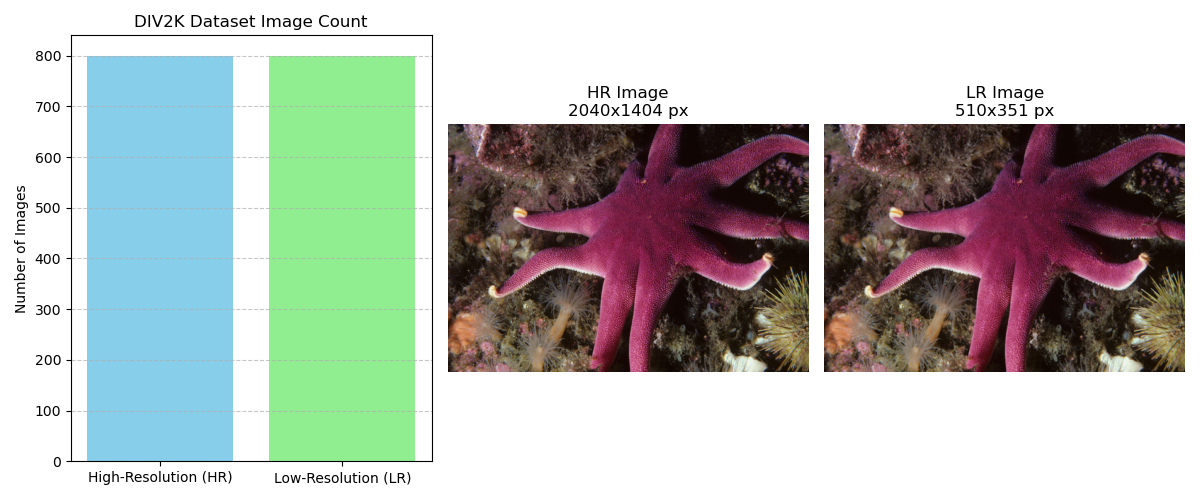
\includegraphics[width=1\textwidth]{image/Figure_1.png} % <-- Update with your actual file path
    \caption{DIV2K Dataset}
    \label{fig:workflow}
\end{figure}

\notocsection{Data Preprocessing}
Before training the model, all images undergo preprocessing to ensure consistency:
\begin{itemize}
    \item \textbf{Resizing}: Images are downsampled to create LR-HR image pairs.
    \item \textbf{Normalization}: Pixel values are scaled to the range $[0, 1]$  depending on the activation function used in the neural network.
    \item \textbf{Data Augmentation}: Techniques such as rotation, flipping, and cropping help in increasing the diversity of the training data.
\end{itemize}
\vspace{0.5cm}

\notocsection{Execution and Designing of GAN}
A Generative Adversarial Network (GAN) is composed of two primary components:

\textbf{1. Generator: }We built a deep generator using Residual-in-Residual Dense Blocks (RRDB), capable of learning fine image textures. It accepts low-resolution (LR) images and upscales them to high-resolution (HR) outputs using learned features and two upsampling layers.
    
\textbf{2. Discriminator:} A deep CNN-based network that classifies between real HR images and those generated by the generator. It is trained adversarially to improve perceptual quality.

\vspace{0.7cm}
    
% \textbf{Loss Functions:}
    
    % \begin{itemize}
    %     \item Perceptual Loss: Implemented using a pre-trained VGG19 network to compute feature-based loss.
        
    %     \item Adversarial Loss: Helps the generator produce more realistic outputs.
        
    %     \item Pixel Loss (L1): Encourages similarity between generated and real images at pixel level.
        
    % \end{itemize}
% We trained the model using the Wasserstein GAN with Gradient Penalty approach to ensure stable training and better visual results. The ESRGAN model was trained for 100 epochs and compared with a CNN baseline to validate its effectiveness.The generator is trained to fool the discriminator while the discriminator learns to better distinguish between real and generated images.

\notocsection{Training and Fine-Tuning}
In this project, we trained the ESRGAN model on the DIV2K dataset in two stages:

\textbf{Initial Training:}

Stabilize the generator before introducing adversarial loss.

Trained the generator alone for 100 epochs using only the L1 (pixel) loss.

\textbf{Settings:}

\begin{itemize}
    \item Optimizer: Adam (learning rate 1e-4, $\beta$₁=0.9, $\beta$₂=0.999)
    \item Batch size: 8
    \item LR scheduling: Reduce by factor of 10 at epoch 50
\end{itemize}

\textbf{Adversarial Fine-Tuning}

Improve perceptual fidelity by introducing the discriminator and perceptual loss.

Jointly trained generator and discriminator for 200 additional epochs.

\textbf{Settings:}

\begin{itemize}
    \item Discriminator updates per generator update: 1
    \item Loss weights: 1.0·L1, 2e-6·Perceptual, 1e-3·Adversarial
    \item Learning rate kept at 1e-4, halved at epoch 100
\end{itemize}


% The training process involves multiple loss functions:
% \begin{itemize}
%     \item \textbf{Adversarial Loss} ($\mathcal{L}_{adv}$): Encourages the generator to produce perceptually realistic images.
%     \item \textbf{Perceptual Loss} ($\mathcal{L}_{perc}$): Uses feature maps from a pretrained network (e.g., VGG) to ensure perceptual similarity.
%     \item \textbf{Content Loss} ($\mathcal{L}_{content}$): Based on pixel-wise differences such as L1 or L2 loss between generated and real images.
% \end{itemize}
% The total loss function is a weighted sum of these components:
% \[
% \mathcal{L}_{total} = \lambda_{adv} \mathcal{L}_{adv} + \lambda_{perc} \mathcal{L}_{perc} + \lambda_{content} \mathcal{L}_{content}
% \]

\notocsection{Evaluation}
The performance of the super-resolution GAN is measured using standard image quality metrics:
\begin{itemize}
    \item \textbf{PSNR (Peak Signal-to-Noise Ratio)}: Measures the ratio between the maximum possible power of a signal and the power of corrupting noise.
    \item \textbf{SSIM (Structural Similarity Index)}: Evaluates the similarity between the generated and ground truth images based on luminance, contrast, and structure.
    o further validate image fidelity, we converted grayscale versions of the SR and HR images into binary representations and computed the following:

\item \textbf{Precision:}
Precision evaluates the proportion of predicted positive pixels that were actually correct. High precision indicates fewer false positives in the generated images.

\item \textbf{Recall:}
Recall measures the ability of the model to capture all the relevant high-frequency details. Our model achieved high recall values, showing it effectively preserved essential visual information.

\item \textbf{F1 Score:}
F1 Score is the harmonic mean of precision and recall, providing a balance between the two. A strong F1 score in our results reflects the overall accuracy of the GAN-generated images in replicating the ground truth.
\end{itemize}
% Higher PSNR and SSIM values typically indicate better quality reconstruction.
\vspace{0.5cm}

% \section{Application and Validation}
% Once trained and evaluated, the model can be deployed in practical applications:
% \begin{itemize}
%     \item \textbf{Medical Imaging}: Enhancing MRI or CT scans for better diagnosis.
%     \item \textbf{Surveillance Systems}: Improving the clarity of footage captured from low-resolution security cameras.
%     \item \textbf{Streaming Platforms}: Enhancing video quality for improved viewing experience in low bandwidth conditions.
% \end{itemize}
% \begin{figure}[h!]
%     \centering
%     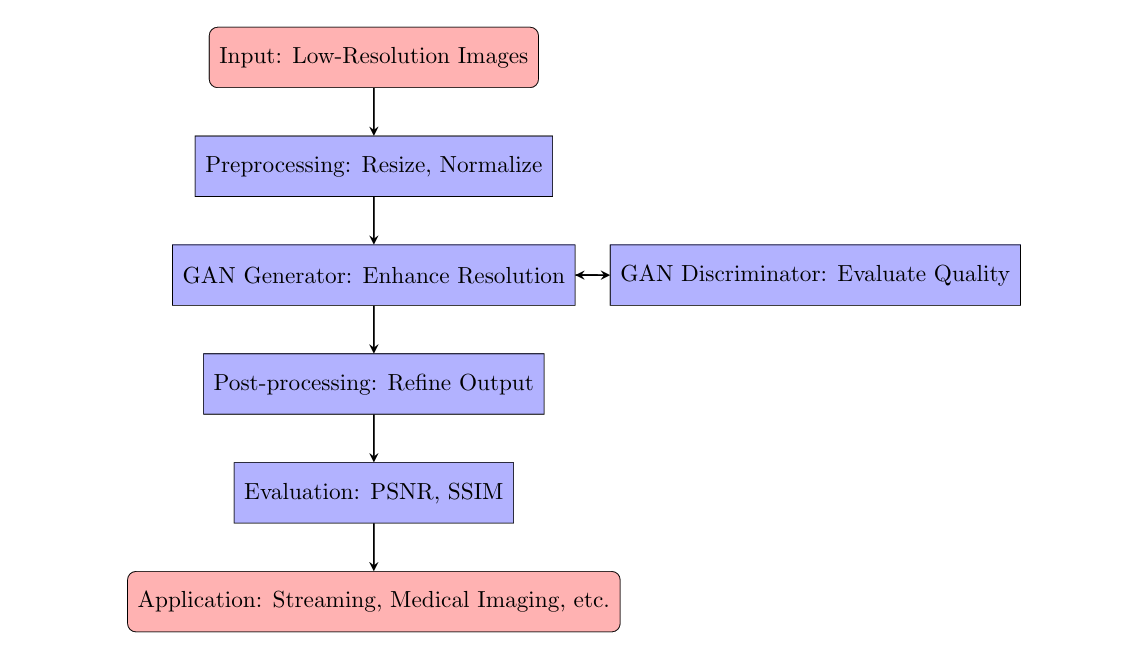
\includegraphics[width=1\textwidth]{workflow.png} % <-- Update with your actual file path
%     \caption{Workflow diagram of the proposed super-resolution methodology.}
%     \label{fig:workflow}
% \end{figure}
% The effectiveness of the model can be validated by comparing the performance of real-world tasks (e.g., object detection accuracy) before and after applying super-resolution.


% \begin{center}

% \begin{tikzpicture}[node distance=1.8cm]

% % Nodes
% \node (start) [startstop] {Input: Low-Resolution Images};
% \node (preprocess) [process, below of=start] {Preprocessing: Resize, Normalize};
% \node (generator) [process, below of=preprocess] {GAN Generator: Enhance Resolution};
% \node (discriminator) [process, right of=generator, xshift=5.5cm] {GAN Discriminator: Evaluate Quality};
% \node (postprocess) [process, below of=generator] {Post-processing: Refine Output};
% \node (finetuning) [process, below of=postprocess] {Post-processing: Refine Output};
% \node (evaluate) [process, below of=postprocess] {Evaluation: PSNR, SSIM};
% % \node (application) [startstop, below of=evaluate] {Application: Streaming, Medical Imaging, etc.};

% % Arrows
% \draw [arrow] (start) -- (preprocess);
% \draw [arrow] (preprocess) -- (generator);
% \draw [arrow] (generator) -- (postprocess);
% \draw [arrow] (postprocess) -- (finetuning);
% \draw [arrow] (finetuning) -- (evaluate);
% % \draw [arrow] (evaluate) -- (application);
% \draw [arrow] (generator.east) -- (discriminator.west);
% \draw [arrow] (discriminator.west) ++(-0.2,0) |- (generator.east);

% \end{tikzpicture}
% \end{center}
\notocsection{GAN Implementation}
In this project, we implemented an Enhanced Super-Resolution Generative Adversarial Network (ESRGAN) to convert low-resolution images into high-resolution outputs. The implementation involved the following major steps:

\begin{itemize}
    \item \textbf{Generator Network:} Designed using Residual-in-Residual Dense Blocks (RRDB), the generator takes low-resolution images as input and learns to produce perceptually accurate high-resolution images. It includes deep convolutional layers, skip connections, and upsampling blocks to preserve fine details.
    
    \item \textbf{Discriminator Network:} A convolutional neural network (CNN) that distinguishes between real high-resolution images and generated images. It guides the generator to produce more realistic outputs through adversarial training.
    
    \item \textbf{Loss Functions:} The model was trained using a combination of adversarial loss, L1 loss, and VGG perceptual loss. This ensured that the generated images were not only visually realistic but also structurally similar to the original high-resolution images.

    \textbf{1. Adversarial Loss (0.866):} Indicates how effectively the generator is able to fool the discriminator. A positive value shows that the generator is learning meaningful features and successfully confusing the discriminator.

\textbf{2. Critic Loss / Wasserstein Distance (25.4):} Represents the ability of the discriminator to distinguish between real and generated images. Higher values suggest better discrimination capability, which guides the generator to improve further.

\textbf{3. Gradient Penalty (0.894):} Used to enforce the Lipschitz constraint in WGAN-GP. A stable and low gradient penalty ensures smoother and more stable training dynamics.

\textbf{4. L1 Loss (0.00235): }Measures the average pixel-wise error between generated and real high-resolution images. A low L1 loss indicates high fidelity in pixel-level reconstruction.

\textbf{5. VGG Perceptual Loss (2.55):} Quantifies the perceptual similarity using high-level features extracted from a pre-trained VGG19 network. Lower values imply that the generated images closely resemble the ground truth in terms of content and texture.
\vspace{0.5cm}
\end{itemize}


% \begin{center}
% \begin{tikzpicture}[node distance=1.9cm]

% % Node styles (if not already defined in your preamble)
% \tikzstyle{startstop} = [rectangle, rounded corners, minimum width=3cm, minimum height=1cm,text centered, draw=black, fill=blue!20]
% \tikzstyle{process} = [rectangle, minimum width=3cm, minimum height=1cm, text centered, draw=black, fill=orange!30]
% \tikzstyle{arrow} = [thick,->,>=stealth]

% % Nodes
% \node (start) [startstop] {Input: Low-Resolution Images};
% \node (preprocess) [process, below of=start] {Preprocessing: Resize, Normalize};
% \node (generator) [process, below of=preprocess] {GAN Generator: Enhance Resolution};
% \node (discriminator) [process, right of=generator, xshift=6.1cm] {GAN Discriminator: Evaluate Quality};
% \node (postprocess) [process, below of=generator] {Training and Fine-Tuning};
% \node (evaluate) [process, below of=postprocess] {Evaluation: PSNR, SSIM};
% \node (implementation) [process, below of=evaluate] {GAN Implementation};

% % Arrows
% \draw [arrow] (start) -- (preprocess);
% \draw [arrow] (preprocess) -- (generator);
% \draw [arrow] (generator) -- (postprocess);
% \draw [arrow] (postprocess) -- (evaluate);
% \draw [arrow] (evaluate) -- (implementation);
% \draw [arrow] (generator.east) -- (discriminator.west);
% \draw [arrow] (discriminator.south) |- ++(0,-0.6) -| (generator.south);

% \end{tikzpicture}
% \end{center}
% \hspace{3cm} \large{:- Workflow of SRGAN}
% \vspace{0.6cm}

\begin{figure}[h!]
    \centering
    \includegraphics[width=1\textwidth]{Fig3.2.png} % <-- Update with your actual file path
    \caption{Workflow of SRGAN}
    \label{fig:workflow}
\end{figure}

\noindent The methodology for the proposed GAN-based super-resolution system is illustrated in the workflow diagram above. It outlines the key steps, from dataset acquisition to evaluation and GAN Implementation.


The process begins with the acquisitions and preprocessing of low-resolution images. These images are then passed through a GAN-based model, where the generator attempts to reconstruct high-resolution images while the discriminator evaluates their realism. The model is trained using a combination of adversarial, perceptual, and pixel-wise losses. Finally, the results are evaluated using metrics such as PSNR and SSIM to validate performance.

\large\textbf{Implementation}

\begin{lstlisting}[language=Python, caption={ESRGAN Inference Code}]
import os
for dirname, _, filenames in os.walk('/kaggle/input'):
    print(dirname)

from PIL import Image

import numpy as np
from tqdm import tqdm

import cv2
import matplotlib.pyplot as plt

import torch
import torch.nn as nn
from torch.utils.data import Dataset, DataLoader
import torchvision
import torchvision.transforms as transforms
from torchvision.models import vgg19

import albumentations as A
from albumentations.pytorch import ToTensorV2

class SRDataset(Dataset):
    def __init__(self, root_dir, lowres_transform, highres_transform, both_transform):
        super(SRDataset, self).__init__()

        self.root_dir = root_dir

        self.lowres_transform = lowres_transform
        self.highres_transform = highres_transform
        self.both_transform = both_transform

        self.list_of_files = os.listdir(os.path.join(root_dir))

    def __len__(self):
        return len(self.list_of_files)

    def __getitem__(self, index):
        image = cv2.imread(os.path.join(self.root_dir, self.list_of_files[index]))
        image = cv2.cvtColor(image, cv2.COLOR_BGR2RGB)

        image = self.both_transform(image=image)['image']
        low_res_image = self.lowres_transform(image=image)['image']
        high_res_image = self.highres_transform(image=image)['image']

        return low_res_image, high_res_image

class ConvBlock(nn.Module):
    def __init__(self, in_channels, out_channels, use_act, kernel_size=3, stride=1, padding=1):
        super().__init__()
        self.cnn = nn.Conv2d(
            in_channels,
            out_channels,
            kernel_size=kernel_size,
            stride=stride,
            padding=padding
        )
        self.act = nn.LeakyReLU(0.2, inplace=True) if use_act else nn.Identity()

    def forward(self, x):
        return self.act(self.cnn(x))

class UpsampleBlock(nn.Module):
    def __init__(self, in_channels, scale_factor=2):
        super().__init__()
        self.upsample = nn.Upsample(scale_factor=scale_factor, mode="nearest")
        self.conv = nn.Conv2d(in_channels, in_channels, 3, 1, 1, bias=True)
        self.act = nn.LeakyReLU(0.2, inplace=True)

    def forward(self, x):
        return self.act(self.conv(self.upsample(x)))



class DenseResidualBlock(nn.Module):
    def __init__(self, in_channels, channels=32, residual_beta=0.2):
        super().__init__()
        self.residual_beta = residual_beta
        self.blocks = nn.ModuleList()

        for i in range(5):
            self.blocks.append(
                ConvBlock(
                    in_channels + channels*i,
                    channels if i <= 3 else in_channels,
                    kernel_size=3,
                    stride=1,
                    padding=1,
                    use_act=True if i <=3 else False,
                )
            )

    def forward(self, x):
        new_inputs = x
        for block in self.blocks:
            out = block(new_inputs)
            new_inputs = torch.cat([new_inputs, out], dim=1)

        return self.residual_beta * out + x

class RRDB(nn.Module):
    def __init__(self, in_channels, residual_beta=0.2):
        super().__init__()
        self.residual_beta = residual_beta
        self.rrdb = nn.Sequential(*[DenseResidualBlock(in_channels) for _ in range(3)])

    def forward(self, x):
        return self.rrdb(x) * self.residual_beta + x

class Generator(nn.Module):
    def __init__(self, in_channels=3, num_channels=64, num_blocks=23):
        super().__init__()
        self.initial = nn.Conv2d(
            in_channels=in_channels,
            out_channels=num_channels,
            kernel_size=3,
            stride=1,
            padding=1,
            bias=True
        )
        self.residuals = nn.Sequential(*[RRDB(num_channels) for _ in range(num_blocks)])
        self.conv = nn.Conv2d(num_channels, num_channels, kernel_size=3, stride=1, padding=1)
        self.upsamples = nn.Sequential(
            UpsampleBlock(num_channels),
            UpsampleBlock(num_channels)
        )
        self.final = nn.Sequential(
            nn.Conv2d(num_channels, num_channels, kernel_size=3, stride=1, padding=1, bias=True),
            nn.LeakyReLU(0.2, inplace=True),
            nn.Conv2d(num_channels, in_channels, kernel_size=1, stride=1, padding=0, bias=True)
        )

    def forward(self, x):
        initial = self.initial(x)
        out = self.residuals(initial)
        out = self.conv(out) + initial
        out = self.upsamples(out)
        out = self.final(out)
        return out

class Discriminator(nn.Module):
    def __init__(self, in_channels=3, features=(64, 64, 128, 128, 256, 256, 512, 512)):
        super().__init__()

        self.in_channels = in_channels
        self.features = list(features)

        blocks = []

        for idx, feature in enumerate(self.features):
            blocks.append(
                ConvBlock(
                    in_channels=in_channels,
                    out_channels=feature,
                    kernel_size=3,
                    stride=1 + idx % 2,
                    padding=1,
                    use_act=True
                )
            )
            in_channels=feature

        self.blocks = nn.Sequential(*blocks)

        self.classifier = nn.Sequential(
            nn.AdaptiveAvgPool2d((6, 6)),
            nn.Flatten(),
            nn.Linear(in_features=512*6*6, out_features=1024),
            nn.LeakyReLU(0.2, inplace=True),
            nn.Linear(in_features=1024, out_features=1)
        )
        self.sigmoid = nn.Sigmoid()

    def forward(self, x):
        features = self.blocks(x)
        out = self.classifier(features)
        # out = self.sigmoid(out)
        return out

def init_weights(model, scale=0.1):
    for m in model.modules():
        if isinstance(m, nn.Conv2d):
            nn.init.kaiming_normal_(m.weight.data)
            m.weight.data *= scale
        elif isinstance(m, nn.Linear):
            nn.init.kaiming_normal_(m.weight.data)
            m.weight.data *= scale

def test_size():
    gen = Generator()
    disc = Discriminator()
    low_res = 24
    x = torch.randn((5, 3, low_res, low_res))
    gen_out = gen(x)
    disc_out = disc(x)

    print(gen_out.shape)
    print(disc_out.shape)

test_size()
\end{lstlisting}
